\documentclass[11pt]{aastex}
\usepackage{geometry}                % See geometry.pdf to learn the layout options. There are lots.
\geometry{letterpaper}                   % ... or a4paper or a5paper or ... 
%\geometry{landscape}                % Activate for for rotated page geometry
%\usepackage[parfill]{parskip}    % Activate to begin paragraphs with an empty line rather than an indent
\usepackage{graphicx}
\usepackage{amssymb}
\usepackage{epstopdf}
\DeclareGraphicsRule{.tif}{png}{.png}{`convert #1 `dirname #1`/`basename #1 .tif`.png}

\title{The Mass-Radius Relation for 71 Exoplanets with $\rpl < 7 \rearth$}
\author{L. M. Weiss \& G. W. Marcy}
%\date{}                                           % Activate to display a given date or no date

%---------------------------- Physical Quantities ------------------------------------%
\newcommand{\kms}{\ensuremath{\rm km\,s^{-1}}}
\newcommand{\ms}{\ensuremath{\rm m\,s^{-1}}}
\newcommand{\mse}{\ensuremath{\rm m\,s^{-1}}}
\newcommand{\gcmc}{\ensuremath{\rm g\,cm^{-3}}}
\newcommand{\gcc}{\gcmc}
\newcommand{\fluxunit}{\ensuremath{\rm erg\,s^{-1}\,cm^{-2}}}
\newcommand{\rhk}{\ensuremath{R^{\prime}_{\rm HK}}}	% Activity index R'_HK
\newcommand{\logrhk}{\ensuremath{\log\rhk}}		% log of R'_HK

\newcommand{\teff}{\ensuremath{T_{\rm eff}}}
\newcommand{\logg}{\ensuremath{\log{g}}}
\newcommand{\vsini}{\ensuremath{v \sin{i}}}
\newcommand{\feh}{[Fe/H]}
\newcommand{\logl}{\ensuremath{\log{L}}}

\newcommand{\rsun}{\ensuremath{R_\sun}}
\newcommand{\msun}{\ensuremath{M_\sun}}
\newcommand{\lsun}{\ensuremath{L_\sun}}

\newcommand{\rstar}{\ensuremath{R_\star}}
\newcommand{\mstar}{\ensuremath{M_\star}}
\newcommand{\loggstar}{\ensuremath{\logg_\star}}
\newcommand{\lstar}{\ensuremath{L_\star}}
\newcommand{\astar}{\ensuremath{a_\star}}
\newcommand{\loglstar}{\ensuremath{\log{L_\star}}}
\newcommand{\rhostar}{\ensuremath{\rho_\star}}

\newcommand{\rpl}{\ensuremath{R_{\rm P}}}
\newcommand{\mpl}{\ensuremath{M_{\rm P}}}
\newcommand{\lpl}{\ensuremath{L_{\rm P}}}
\newcommand{\rhopl}{\ensuremath{\rho_{\rm P}}}
\newcommand{\loggpl}{\ensuremath{\logg_{\rm P}}}
\newcommand{\teq}{\ensuremath{T_{\rm eq}}}

\newcommand{\rjup}{\ensuremath{R_{\rm J}}}
\newcommand{\mjup}{\ensuremath{M_{\rm J}}}
\newcommand{\rhojup}{\ensuremath{\rho_{\rm J}}}
\newcommand{\rearth}{\ensuremath{R_\earth}}
\newcommand{\mearth}{\ensuremath{M_\earth}}
\newcommand{\fearth}{\ensuremath{F_\earth}}

\newcommand{\msini}{\ensuremath{m \sin{i}}}
\newcommand{\mplsini}{\ensuremath{\mpl\sin{i}}}

\newcommand{\npl}{225~} % The number of exoplanets used to determine the MRF relation
\newcommand{\nhires}{42~} % The number of transiting planets in the HIRES paper
\newcommand{\nlm}{71~}
\newcommand{\rspecial}{7 \rearth}

\begin{document}
\maketitle
\section{Introduction}
%\subsection{}

The Kepler Mission has found an arbundance of planets with  $R < 4\rearth$.  However, in many systems, it is difficult to measure the masses of such small planets because the gravitational acceleration these planets induce on their host stars or neighboring planets is too small to detect with current telescopes and instruments.  How can we determine the composition of these planets?  To understand the nature of small planets, we reverse the question: how do the mass of a planet, its composition, and the incident stellar flux from its star affect the radius of a planet?  

Our work \citep{Weiss2013} has shown that for planets between $\sim$20 and thousands of Earth masses, we can predict the radius of a planet from its mass and incident stellar flux, suggesting that planets of a given mass have a particular composition.  However, below $\sim$20 \mearth, the large apparent scatter makes predicting planet radius harder.  At 10 Earth masses, planets can have a radius of 2-8 \rearth, which spans a range in density from less dense than water to solid iron.

There are two explanations for the large apparent scatter in planet radius: either errors in radius and/or mass are underestimated for 
planets below 20 \mearth, or the (real) scatter in radius indicates a diversity of planet compositions.   Identifying whether this apparent scatter is real or not is one of the most pressing issues in understanding planetary compositions today.  Does the mass of a planet uniquely determine a planet�s composition, or is there diversity of the rock to volatile ratio at a given mass?  If the scatter is only apparent, then it is possible that there is a one-to-one correspondence between planet mass and composition below 20 \mearth.  However, if the scatter is real, then there must be a diversity of planet compositions at a given mass below 20 \mearth.  Further refinements to the measurements of planet masses, especially below 20 \mearth, is necessary to test to what extent the apparent scatter of planetary masses at a given radius is real.


\section{Justification for a Mass-Radius Relation for Low-Mass Exoplanets}
Is there a correlation between planet mass and radius for small exoplanets?  By eye, we might judge that there is a correlation, but what is the probability that we have fooled ourselves into believing there is a correlation when in fact there is none?

To answer this question, I calculated the probability that the data were uncorrelated.  First, I calculated the correlation coefficient (Pearson R test) r = 0.61.  For r = 0.61, the Student t value is 6.38.  There are 71 planets with $\rpl < \rspecial$, so there are 69 degrees of freedom in this sample.  What is the probability that among data with 69 degrees of freedom, we find a Student t value of 6.38 if the data are uncorrelated?  According to a Wolfram Alpha calculation, the probability of obtaining $t \ge 6.38$ for 69 degrees of freedom, given that the data are really uncorrelated, is $3.56 \times 10^{-8}$.  We can safely say that the masses and radii of small planets are correlated.

Does this correlation also exist for planets with $\rpl < 4 \rearth$?  There are 58 planets smaller than 4 \rearth, leaving 56 degrees of freedom.  The Pearson R coefficient is 0.51, and the Student t value is 4.4.  The probability that these data are uncorrelated is $8.4 \times 10^{-5}$.  Thus, the masses and radii of planets between the sizes of Earth and Neptune are correlated.

\section{The Updated Mass-Radius Relation for Small Exoplanets}
Now that we have determined that a correlation between planet mass and radius exists, what is the best way to model the relation between exoplanet mass and radius?  Figure \ref{fig:rm_7} suggests that the data can be fit with a line; a more complicated fit is not warranted.  To check this, we try a traditional power-law fit and obtain $\mpl \propto \rpl^1$ as the best result.

The best linear fit to the data for \rpl $<$ \rspecial is:
$$
\mpl/\mearth = -0.15 +  3.01 \rpl/\rearth
$$
There are 71 exoplanets in this sample.  The reduced $\chi^2$=5.90, and the RMS is 9.37 \mearth.

However, we notice in Figure \ref{fig:rbin} that the weighted mean masses might follow a different trend above and below 4 \rearth.  Also, there are very few planets with $4 < \rpl < 7$, and the scatter in their masses is large.  This motivates us to do a linear fit between mass and radius on the subsample of exoplanets with \rpl $<$ 4, obtaining:
$$
\mpl/\mearth = 1.01 + 2.33 \rpl/\rearth
$$
There are 58 exoplanets in this sample.  The reduced $\chi^2$=3.74, and the RMS is 5.01\mearth.

This update benefits from (1) the masses of \nhires low-mass planets recently characterized in \citet{Marcy2013}, (2) additional planets of all masses added to exoplanets.org between 27 September 2012 and [use most recent update] 2013, and (3) refined planet and stellar parameters for several systems, including 55 Cnc e (cite), Kepler-11 \citep{Lissauer2013}, GJ 3470 \citep{Demory2013}, HD 97658 b \citep{Dragomir2013}, [... other systems].

\subsection{Using Negative Planet Masses for Statistical Soundness}
\citet{Marcy2013} allow ``negative" planet masses as Keplerian orbital solutions to avoid the Lutz-Kelker bias.  A ``negative" planet mass arises when, given the orbital period and phase determined by the transit, the RV data have the opposite sign from what is expected.  This yields a negative semi-amplitude $K$ in the orbital solution, which results in a negative planet mass.  
	In a traditional analysis, the uncertainties in the RVs and the number of measurements combine to determine an upper limit to the planet mass.  However, upper limits to planet masses are difficult to use statistically.  The artifice of a negative planet mass allows the population of small planets to be treated statistically.  Since there is no bias toward large or small planet masses in our sample, we can take the weighted mean mass of planets of a given radius.
	
\begin{comment}
\subsection{Determining the MRF Relation}
Figure \ref{fig:mrf} shows the masses and radii of \npl exoplanets.  In Table \ref{tab:mrf}, we present the mass and radius of exoplanets, and the incident flux from the host star, that we used in determining the updated mass-radius flux relation.  The parameters listed in this table are those obtained from exoplanets.org, except where marked otherwise.  (Order table by discovery date for easy comparison with previous and future work?)

In this paper, we use a physically motivated relation between mass, radius, and incident flux.  We assume that there exists a mass-radius relation of the form $\rpl \propto A \times \mpl^B$ for planets that receive little or no incident flux.  We then ask how the incident flux from the host star onto the planet will affect the planet's radius.

\subsubsection{Giant Planets}
For giant planets, high incident flux is correlated with larger planet radii \citep{Weiss2013}.  The standard interpretation (cite lots of stuff) is that incident flux from the host star inflates the gaseous layers of giant planets, and/or slows their contraction.  Basically, the total energy from the star over the lifetime of the planet goes as
$$
E_{star} \propto F \Delta t \pi \rpl^2.
$$
where $F$ is the incident flux, $\Delta t$ is the total time $F$ shines on the planet, and $\pi \rpl^2$ is the cross-sectional area of the planet receiving the flux.

The stellar energy does work on the planet to lift gaseous layers from radius $R$ to $R + \Delta R$, resulting in a total work done equal to
$$
W = \frac{d}{dR}\left(\frac{G\mpl^2}{R}\right) \Delta R
$$
where...
Equating the stellar energy to the work done on the planet, 
$$
F \Delta t \pi \rpl^2 \propto \frac{d}{dR}\left(\frac{G\mpl^2}{R}\right) \Delta R
$$
\end{comment}
%% The values (usually only l,r and c) in the last part of
%% \begin{deluxetable}{} command tell LaTeX how many columns
%% there are and how to align them.
\begin{deluxetable}{lllllll}

%% Keep a portrait orientation


%% Over-ride the default font size
%% Use 10pt
\tabletypesize{\tiny}

\tablewidth{0pt} %to over-ride the default table width.
%% If you are unhappy with the default look at the end of the
%% *.log file to see what the default was set at before adjusting
%% this value.

%% This is the title of the table.
\tablecaption{Exoplanets with Measured Mass and Radius}
%% This command over-rides LaTeX's natural table count
%% and replaces it with this number.  LaTeX will increment 
%% all other tables after this table based on this number
\tablenum{1}
\label{tab:mrf}

%% The \tablehead gives provides the column headers.  It
%% is currently set up so that the column labels are on the
%% top line and the units surrounded by ()s are in the 
%% bottom line.  You may add more header information by writing
%% another line between these lines. For each column that requries
%% extra information be sure to include a \colhead{text} command
%% and remember to end any extra lines with \\ and include the 
%% correct number of &s.
\tablehead{\colhead{Name} & \colhead{Planet Mass} & \colhead{Planet Radius} & \colhead{Incident Flux} & \colhead{Period} & \colhead{First Ref.} & \colhead{Orbital Ref.} \\ 
\colhead{} & \colhead{($M_\earth$)} & \colhead{($R_\earth$)} & \colhead{($F_\earth$)} & \colhead{(d)} & \colhead{} & \colhead{} } 

%% All data must appear between the \startdata and \enddata commands
\startdata
            55 Cnc e &      8.380 &      2.210 &   2439.690 &      0.737 &                     \citet{McArthur2004} &                         \citet{Endl2012}\\ 
           CoRoT-7 b &      5.021 &      1.679 &   1779.433 &      0.854 &             \citet{Queloz2009,Leger2009} &                       \citet{Queloz2009}\\ 
           CoRoT-8 b &     68.673 &      6.389 &     88.184 &      6.212 &                        \citet{Borde2010} &                        \citet{Borde2010}\\ 
           GJ 1214 b &      6.260 &      2.800 &     16.631 &      1.580 &                  \citet{Charbonneau2009} &                       \citet{Carter2011}\\ 
           GJ 3470 b &     13.900 &      4.830 &     38.335 &      3.337 &                      \citet{Bonfils2012} &                      \citet{Demory2013}\\ 
            GJ 436 b &     23.105 &      4.222 &     29.882 &      2.644 &                       \citet{Butler2004} &                       \citet{Maness2007}\\ 
          HAT-P-11 b &     26.231 &      4.730 &     97.355 &      4.888 &                        \citet{Bakos2010} &                        \citet{Bakos2010}\\ 
          HAT-P-26 b &     18.640 &      6.333 &    163.050 &      4.235 &                     \citet{Hartman2011b} &                      \citet{Hartman2011b} \\ 
          HD 97658 b   &  7.862   &  2.340  &  48.052  &   9.491      &                \citet{Howard2011}        &            \citet{Dragomir2013}\\
         Kepler-10 b &      4.539 &      1.416 &   3572.048 &      0.837 &                      \citet{Batalha2011} &                      \citet{Batalha2011}\\ 
         Kepler-11 b &      1.900 &      1.800 &    126.384 &     10.304 &                     \citet{Lissauer2011} &                     \citet{Lissauer2013}\\ 
         Kepler-11 c &      2.900 &      2.870 &     91.413 &     13.025 &                     \citet{Lissauer2011} &                     \citet{Lissauer2011}\\ 
         Kepler-11 d &      7.300 &      3.120 &     43.562 &     22.687 &                     \citet{Lissauer2011} &                     \citet{Lissauer2011}\\ 
         Kepler-11 e &      8.000 &      4.190 &     27.524 &     31.996 &                     \citet{Lissauer2011} &                     \citet{Lissauer2011}\\ 
         Kepler-11 f &      2.000 &      2.490 &     16.745 &     46.689 &                     \citet{Lissauer2011} &                     \citet{Lissauer2011}\\ 
         Kepler-18 b &      6.900 &      2.000 &    462.244 &      3.505 &                      \citet{Borucki2011} &                      \citet{Cochran2011}\\ 
         Kepler-18 c &     17.299 &      5.490 &    163.493 &      7.642 &                      \citet{Borucki2011} &                      \citet{Cochran2011}\\ 
         Kepler-18 d &     16.399 &      6.980 &     67.364 &     14.859 &                      \citet{Borucki2011} &                      \citet{Cochran2011}\\ 
         Kepler-20 b &      8.474 &      1.908 &    343.928 &      3.696 &                      \citet{Borucki2011} &                      \citet{Gautier2012}\\ 
         Kepler-20 c &     15.734 &      3.067 &     81.783 &     10.854 &                      \citet{Borucki2011} &                      \citet{Gautier2012}\\ 
         Kepler-20 d &      7.528 &      2.748 &      5.937 &     77.612 &                      \citet{Borucki2011} &                      \citet{Gautier2012}\\ 
         Kepler-36 b &      4.461 &      1.485 &    217.365 &     13.840 &                      \citet{Borucki2011} &                       \citet{Carter2012}\\ 
         Kepler-36 c &      8.101 &      3.676 &    175.646 &     16.239 &                       \citet{Carter2012} &                       \citet{Carter2012}\\ 
          Kepler-4 b &     24.544 &      4.002 &   1123.918 &      3.213 &                      \citet{Borucki2010} &                      \citet{Borucki2010}\\ 
         Kepler-68 b &      8.300 &      2.310 &    409.092 &      5.399 &                      \citet{Borucki2011} &                    \citet{Gilliland2013}\\ 
         Kepler-68 c &      4.377 &      0.952 &    189.764 &      9.605 &                      \citet{Batalha2013} &                    \citet{Gilliland2013}\\ 
            KOI-94 b &      9.400 &      1.770 &   1155.374 &      3.743 &                        \citet{Weiss2013} &                        \citet{Weiss2013}\\ 
            KOI-94 c &      8.300 &      4.280 &    295.035 &     10.424 &                      \citet{Borucki2011} &                        \citet{Weiss2013}\\ 
            KOI-94 d &    105.000 &     11.400 &    106.760 &     22.343 &                      \citet{Borucki2011} &                        \citet{Weiss2013}\\ 
            KOI-94 e &     38.000 &      6.640 &     32.631 &     54.320 &                      \citet{Borucki2011} &                        \citet{Weiss2013}\\ 
            \hline
KOI-41.01 & 0.85000000 & 2.2000000 & 1156.6217 & 12.815900 & & \\
KOI-41.02 & 7.3400000 & 1.3000000 & 65.166782 & 6.8870500 & &\\
KOI-41.03 & -5.3100000 & 1.6000000 & 85.869041 & 35.333100& & \\
KOI-69.01 & 2.5900000 & 1.5000000 & 172.33078 & 4.7267400 & &\\
KOI-82.01 & 8.9300000 & 2.2000000 & 806.96474 & 16.145700 & &\\
KOI-82.02 & 3.8000000 & 1.2000000 & 147.34753 & 10.311700 & &\\
KOI-82.03 & 8.1200000 & 0.90000000 & 447.82440 & 27.453600 & &\\
KOI-82.04 & -2.4500000 & 0.60000000 & 447.27347 & 7.0714200 & &\\
KOI-82.05 & 0.41000000 & 0.50000000 & 2950.4414 & 5.2869600& & \\
KOI-104.01 & 10.840000 & 3.5000000 & 1189.7862 & 2.5080600 & &\\
KOI-108.01 & 18.690000 & 3.4000000 & 348.15857 & 15.965400 & &\\
KOI-108.02 & -22.540000 & 5.1000000 & 163.05049 & 179.61200 & &\\
KOI-116.01 & 10.440000 & 2.5000000 & 308.73816 & 13.570800 & &\\
KOI-116.02 & 11.170000 & 2.6000000 & 604.88523 & 43.844500 & &\\
KOI-116.03 & 0.15000000 & 0.80000000 & 416.85849 & 6.1648600 & &\\
KOI-116.04 & -13.340000 & 0.90000000 & 298.50217 & 23.980200 & &\\
KOI-122.01 & 13.000000 & 3.4000000 & 1191.9507 & 11.523100 & &\\
KOI-123.01 & 1.3000000 & 2.4000000 & 618.50330 & 6.4816300 & &\\
KOI-123.02 & 2.2200000 & 2.5000000 & 1914.9410 & 21.222700 & &\\
KOI-148.01 & 3.9400000 & 1.9000000 & 1903.1669 & 4.7780000 & &\\
KOI-148.02 & 14.610000 & 2.7000000 & 537.46087 & 9.6739500 & &\\
KOI-148.03 & 7.9300000 & 2.0000000 & 1030.1836 & 42.896100 & &\\
KOI-153.01 & -5.7000000 & 2.2000000 & 1818.3791 & 8.9250700 & &\\
KOI-153.02 & 7.1000000 & 1.8000000 & 439.71133 & 4.7540000 & &\\
KOI-244.01 & 24.600000 & 5.2000000 & 226.04191 & 12.720400 & &\\
KOI-244.02 & 9.6000000 & 2.7000000 & 1560.3683 & 6.2385000 & &\\
KOI-245.01 & -5.9800000 & 1.9000000 & 1367.9423 & 39.792200 & &\\
KOI-245.02 & 3.3500000 & 0.80000000 & 1611.6302 & 21.302000 & &\\
KOI-245.03 & -0.42000000 & 0.30000000 & 2337.2286 & 13.367500 & &\\
KOI-246.01 & 7.8900000 & 2.3000000 & 926.85884 & 5.3987500 & &\\
KOI-246.02 & 2.1800000 & 1.0000000 & 1299.0590 & 9.6050400 & &\\
KOI-261.01 & 8.4600000 & 2.7000000 & 4070.4875 & 16.238500 & &\\
KOI-283.01 & 16.130000 & 2.4000000 & 1637.1673 & 16.092000 & &\\
KOI-283.02 & 17.020000 & 0.80000000 & 909.50346 & 25.516900 & &\\
KOI-292.01 & 3.5100000 & 1.5000000 & 584.57028 & 2.5866400 & &\\
KOI-299.01 & 3.5500000 & 2.0000000 & 1299.4980 & 1.5416800 & &\\
KOI-305.01 & 6.1500000 & 1.5000000 & 142.83632 & 4.6035800 & &\\
KOI-321.01 & 6.3500000 & 1.4000000 & 344.40060 & 2.4262900 & &\\
KOI-321.02 & 2.7100000 & 0.80000000 & 725.85388 & 4.6233200 & &\\
KOI-1442.01 & 0.060000000 & 1.1000000 & 11.621547 & 0.66931000& & \\
KOI-1612.01 & 0.48000000 & 0.80000000 & 1420.2428 & 2.4650200 & &\\
KOI-1925.01 & 2.6900000 & 1.2000000 & 418.26336 & 68.958400 & &\\
\enddata

%% Include any \tablenotetext{key}{text}, \tablerefs{ref list},
%% or \tablecomments{text} between the \enddata and 
%% \end{deluxetable} commands

%% No \tablecomments indicated

%% No \tablerefs indicated

\end{deluxetable}

\begin{figure}[htbp] %  figure placement: here, top, bottom, or page
   \centering
    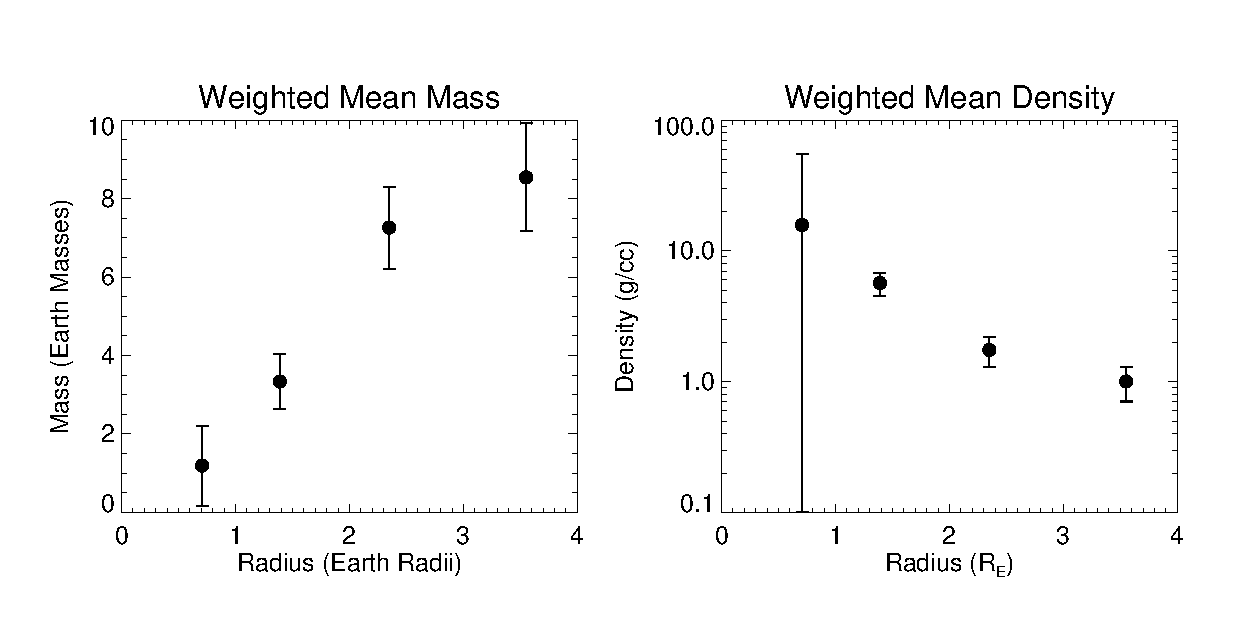
\includegraphics[width=6in]{mr_bin.eps} 
   \caption{The weighted mean mass (left), density (center), and incident flux (right) in bins of 1 \rearth.  The error bars are the weighted uncertainties in the means.}
   \label{fig:rbin}
\end{figure}

\begin{figure}[htbp] %  figure placement: here, top, bottom, or page
   \centering
    \includegraphics[width=6in]{rm_small7.eps} 
   \caption{Mass vs. radius for planets with $\rpl < 7 \rearth$.  Individual planets are represented by black dots, with error bars corresponding to 1$\sigma$ uncertainties.  The dashed line is the best linear fit to the data.  The dotted line is a simple quadratic fit. Red squares represent the weighted mean mass in bins of 1 \rearth, and error bars are the weighted uncertainty in the mean mass (as in Figure \ref{fig:rbin}), to guide the eye.}
   \label{fig:rm_7}
\end{figure}

\begin{figure}[htbp] %  figure placement: here, top, bottom, or page
   \centering
    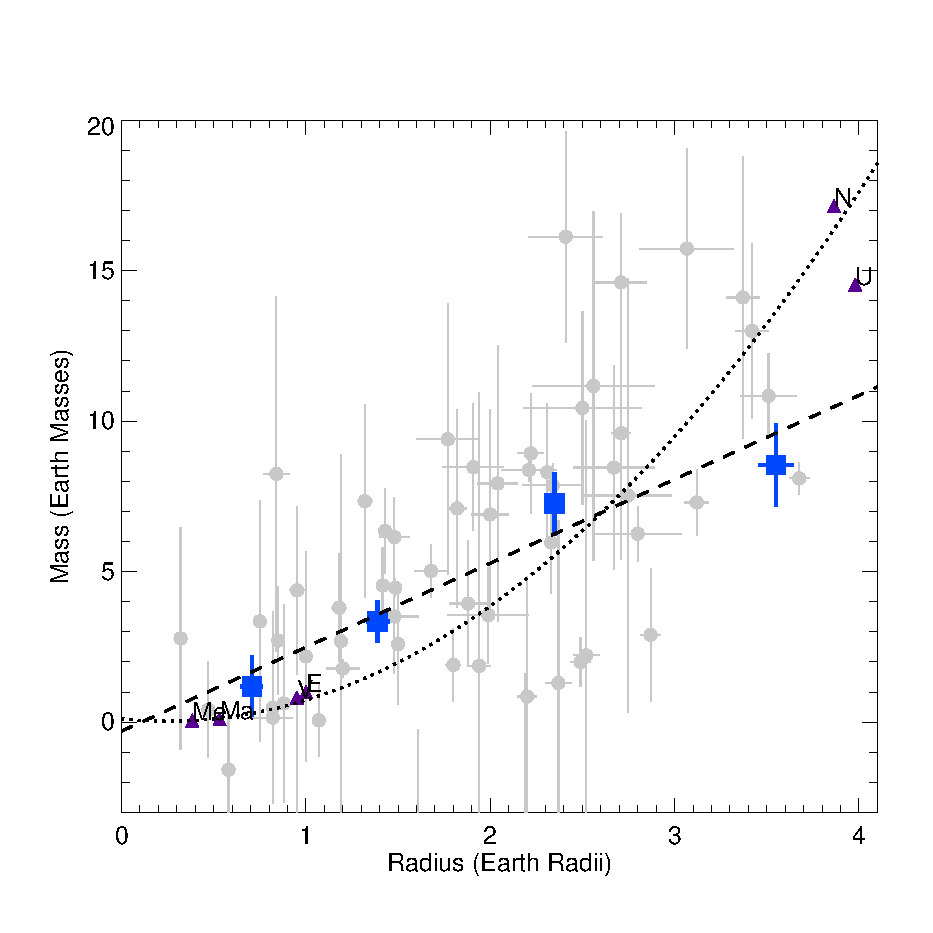
\includegraphics[width=6in]{rm_small4.eps} 
   \caption{Mass vs. radius for planets with $\rpl < 4 \rearth$.  Individual planets are represented by black dots, with error bars corresponding to 1$\sigma$ uncertainties.  The dashed line is the best linear fit to the data.  The dotted line is a simple quadratic fit. Red squares represent the weighted mean mass in bins of 1 \rearth, and error bars are the weighted uncertainty in the mean mass (as in Figure \ref{fig:rbin}), to guide the eye.  The solar system planets are plotted as blue triangles for reference.}
   \label{fig:rm_4}
\end{figure}


\begin{figure}[htbp] %  figure placement: here, top, bottom, or page
   \centering
   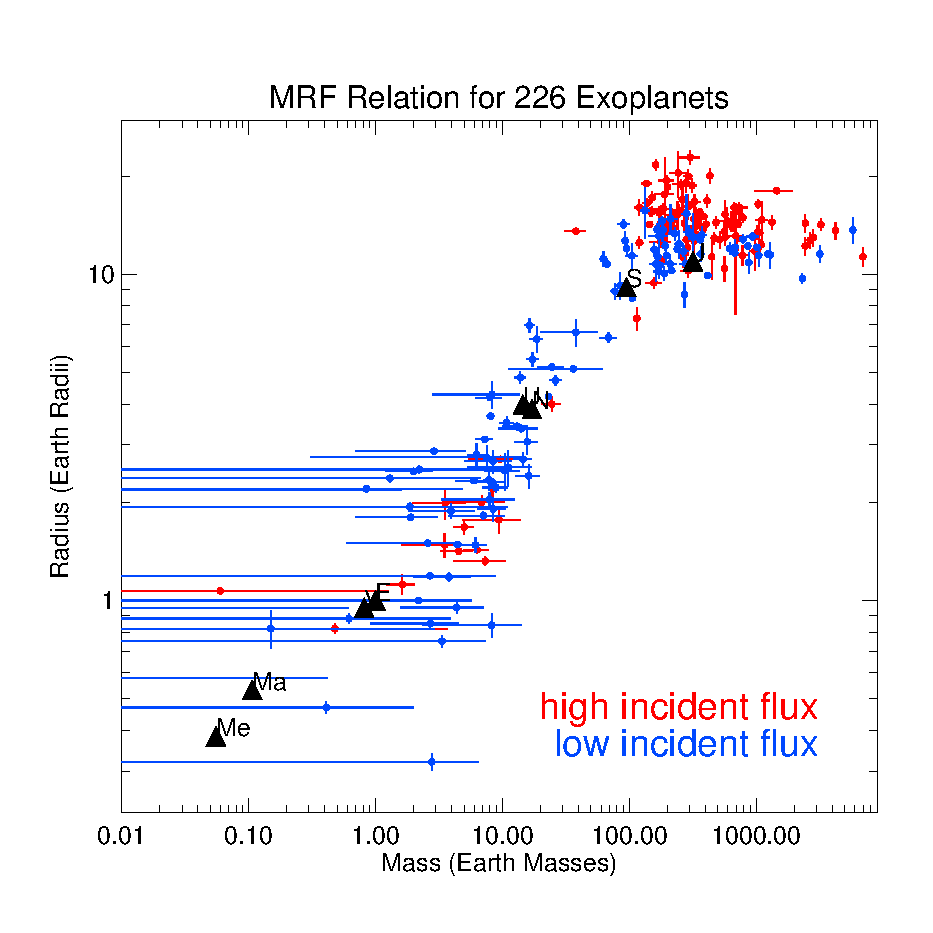
\includegraphics[width=6in]{mrf.eps} 
   \caption{Radius versus mass for exoplanets with measured masses and radii.  Planets receiving lower than the median incident flux are blue; those receiving higher than the median incident flux are red.  A plane was fit to the logspace points to determine a mass-radius-flux relation; the projection of that plane at the median flux is shown (black line).  The Solar System planets are over plotted as black triangles for comparison, although they are not used in determining the fit.}
   \label{fig:mrf}
\end{figure}

\begin{figure}[htbp] %  figure placement: here, top, bottom, or page
   \centering
      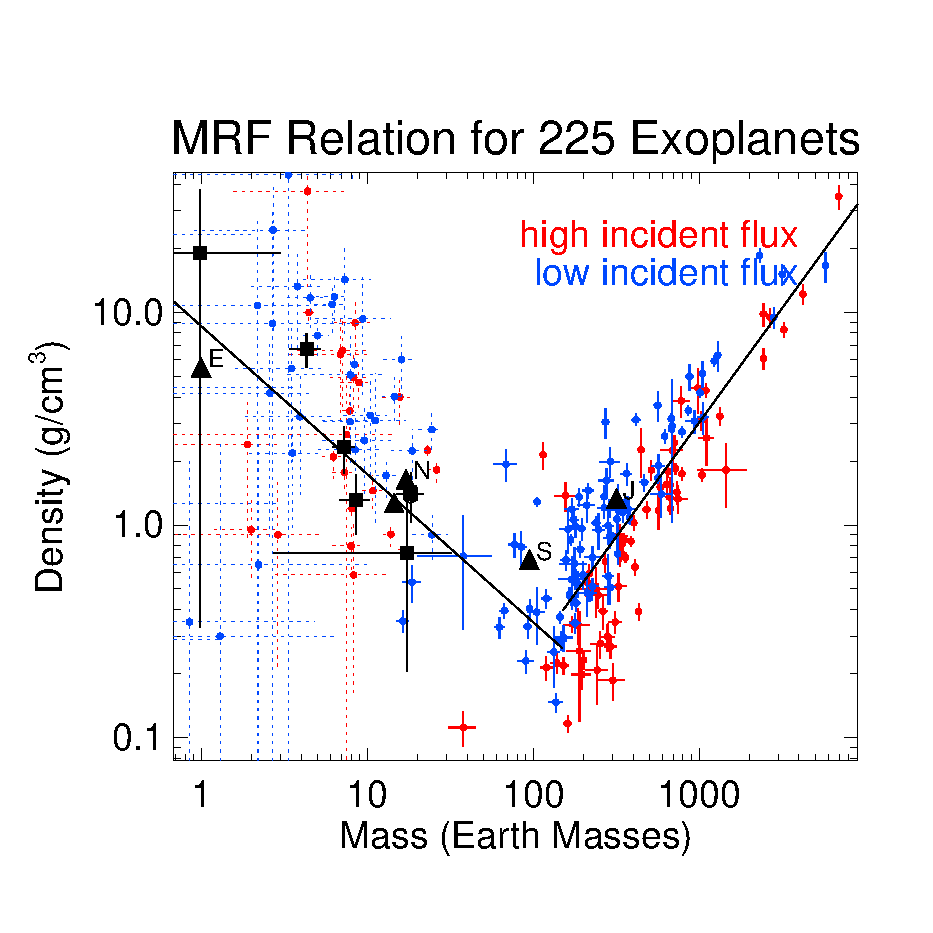
\includegraphics[width=6in]{mdf_fit+22.eps} 
   \caption{Density versus mass for exoplanets with measured masses and radii.  Planets receiving lower than the median incident flux are blue; those receiving higher than the median incident flux are red.  A plane was fit to the logspace points to determine a mass-radius-flux relation; the projection of that plane at the median flux is shown (black line).  The Solar System planets are over plotted as black triangles for comparison, although they are not used in determining the fit.}
   \label{fig:mdf}
\end{figure}

\begin{figure}[htbp] %  figure placement: here, top, bottom, or page
   \centering
      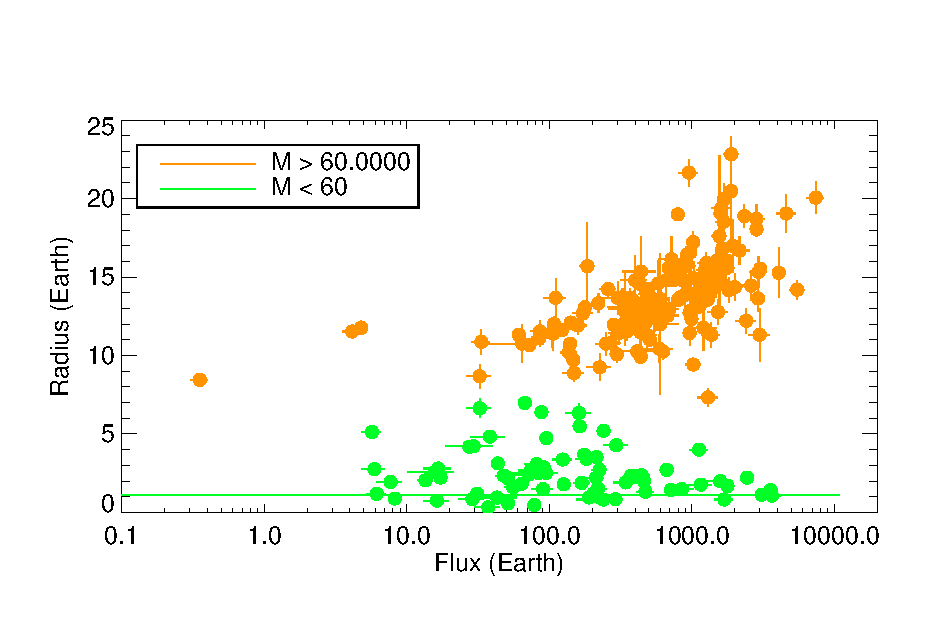
\includegraphics[width=6in]{flux_dependence.eps} 
   \caption{Radius vs. flux for exoplanets with measured masses and radii.  Giant planets are orange; low-mass planets are green.}
   \label{fig:mdf}
\end{figure}

%%%%%%%%%%%%% Discussion %%%%%%%%%%%%%%%%%%%%%%%%%%%%%%%%
\clearpage \section{Discussion}

\bibliography{exoplanet_papers}{}
\bibliographystyle{apj}

\end{document}  